\documentclass{article}
\usepackage[margin=0.7in]{geometry}
\usepackage{amsmath}
\usepackage{amssymb}
\usepackage{bookmark}
\usepackage{graphicx}
\usepackage{float}
\usepackage{hyperref}

\title{Report for Assignment - 2: CS6370 - \\Information Retrieval}
\author{
Harsh Agarwal\\\texttt{CS15BTECH11019}
\and
Sukrut Rao\\\texttt{CS15BTECH11036}
\and
Vishwak Srinivasan\\\texttt{CS15BTECH11043}
}
\date{}

\begin{document}
\maketitle

\section{Introduction}
\begin{flushleft}
TODO
\end{flushleft}

\section{Processing}
\subsection{Task 1: Crawling \& Parsing HTML}
\begin{flushleft}
The first step is to get the book in HTML form, given its URL, and to split it into text files for individual chapters. This involves fetching the book, extracting the text content, and parsing it to remove irrelevant text, such as metadata. Then, the book is separated into chapters. This separation is dependent on the pattern in which chapters are demarcated in each book, and would vary from book to book. Hence, our script for parsing the book assumes a specific book - \textit{\href{https://www.gutenberg.org/files/1342/1342-h/1342-h.htm}{Pride and Prejudice}} by Jane Austen, from \href{https://www.gutenberg.org}{Project Gutenberg}. However, many books on Project Gutenberg are found in very similar formats, and it should be easy to modify the script to cater to other books. The code for fetching, parsing, separating the book into chapters, and saving each chapter in a separate text file can be found in \verb|parse_book.py|.

The procedure is as follows:
\begin{enumerate}
	\item The book in HTML form is fetched from the URL specified. Using the \verb|BeautifulSoup| package, it is converted entirely to text.
	\item Using regular expressions, points of demarcation of individual chapters are found. Similarly, the point demarcating the end of the book is also found.
	\item The book text is split into individual chapters. Each chapter is saved in the separate text file in the output path specified.
	\item The file name for each chapter includes the URL where the book was obtained from. However, forward slashes (\verb|/|) are replaced with the \verb|#| character.
\end{enumerate}

\subsubsection*{Notes}
\begin{enumerate}
	\item To use the script for other Project Gutenberg books, the regular experssions for finding the chapter demarcator and the demarcator for the end of the book may have to be modified.
	\item Usage instructions in further detail can be found in the \verb|README.md| file.
\end{enumerate}
\end{flushleft}
\newpage

\subsection{Task 2}
\subsection{Text processing of the datasets}
\begin{flushleft}
	The following are the steps for processing:
	\begin{enumerate}
		\item Case Folding - convert all documents to lower case. For example: ``I didn't create Atlantis'' becomes ``i didn't create atlantis''.
		\item Removal of special characters and digits - all special characters (quotes, commas, apostrophes, fullstops, etc.) and digits (0 to 9) were removed. This meant that at the end of this step we had nothing but raw text composed of alphabets alone. For example: ``don't'' becomes ``dont'' and ``ariane-5'' becomes ``ariane''.
		\item Removal of stop words - using \texttt{NLTK}'s corpus of stop words, this was easy.
		\item Lemmatization - for this we used \texttt{NLTK}'s \texttt{WordNetLemmatizer}.
	\end{enumerate}
\end{flushleft}

\section{Plots, Top 20 words and Observations - Chapter Wise}
\subsection{Plots}
\begin{flushleft}
	The following are the frequency distribution plots obtained for 10 out of 62 chapters. 
	\begin{figure}[H]
		\begin{minipage}{0.45\linewidth}
			\centering
			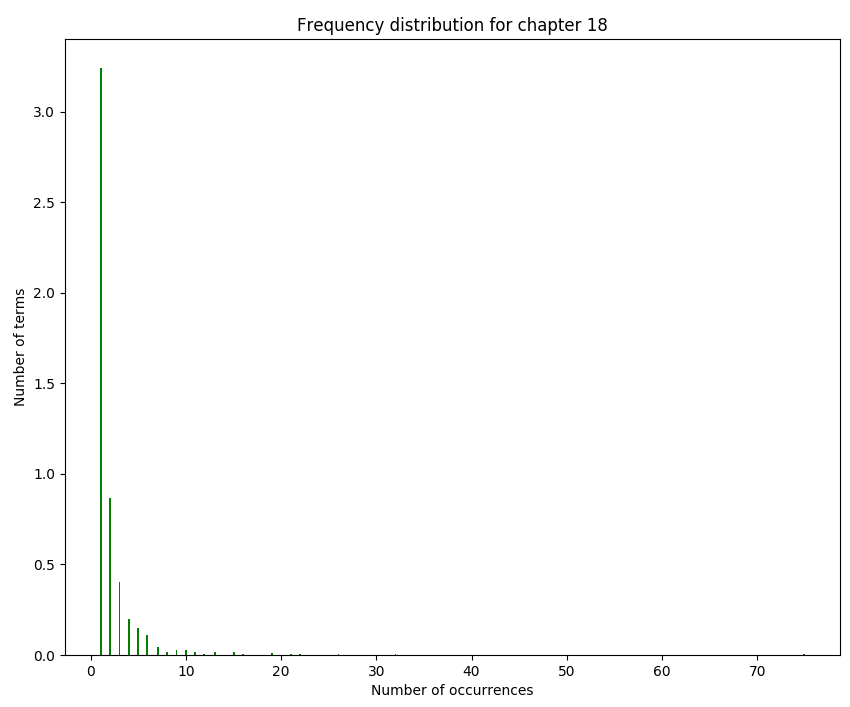
\includegraphics[width=0.75\textwidth]{./images/1-chapter_wise-frequency.png}
			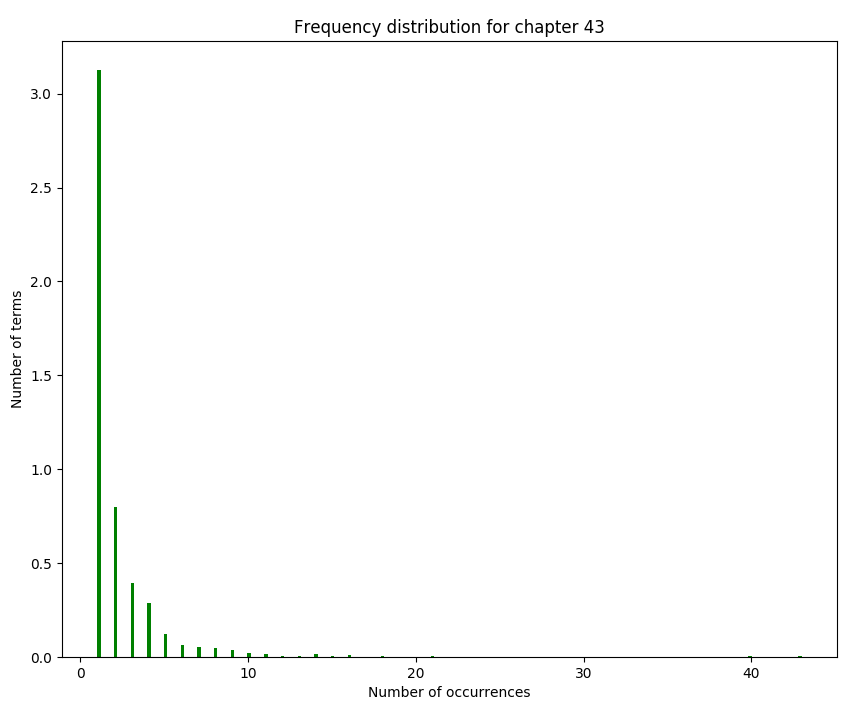
\includegraphics[width=0.75\textwidth]{./images/2-chapter_wise-frequency.png}
			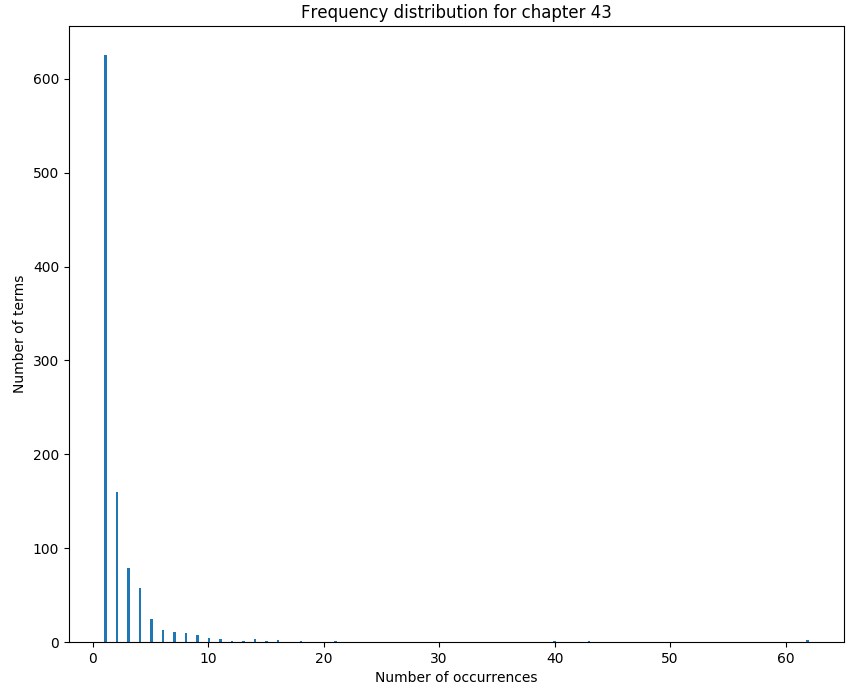
\includegraphics[width=0.75\textwidth]{./images/3-chapter_wise-frequency.png}
			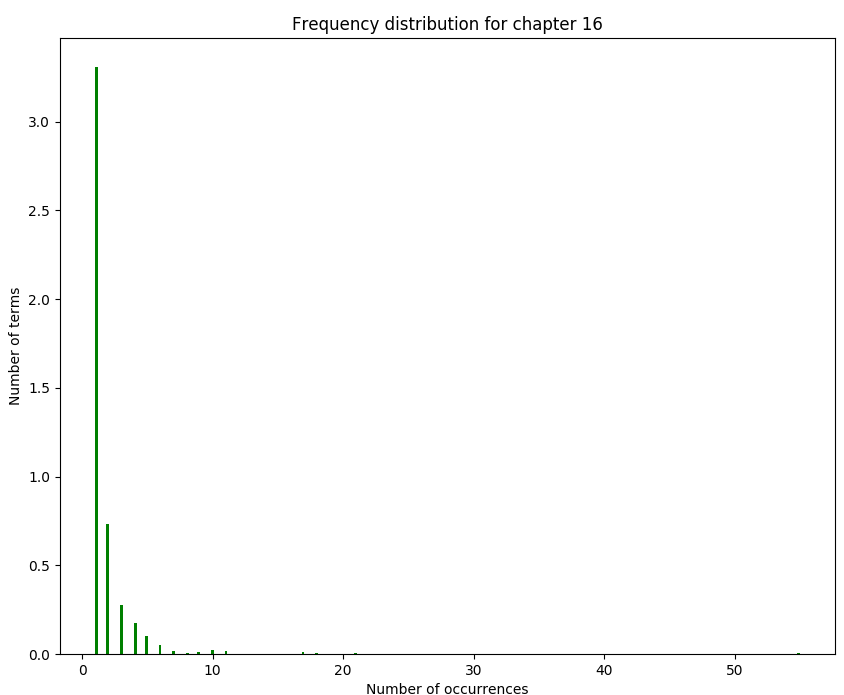
\includegraphics[width=0.75\textwidth]{./images/4-chapter_wise-frequency.png}
			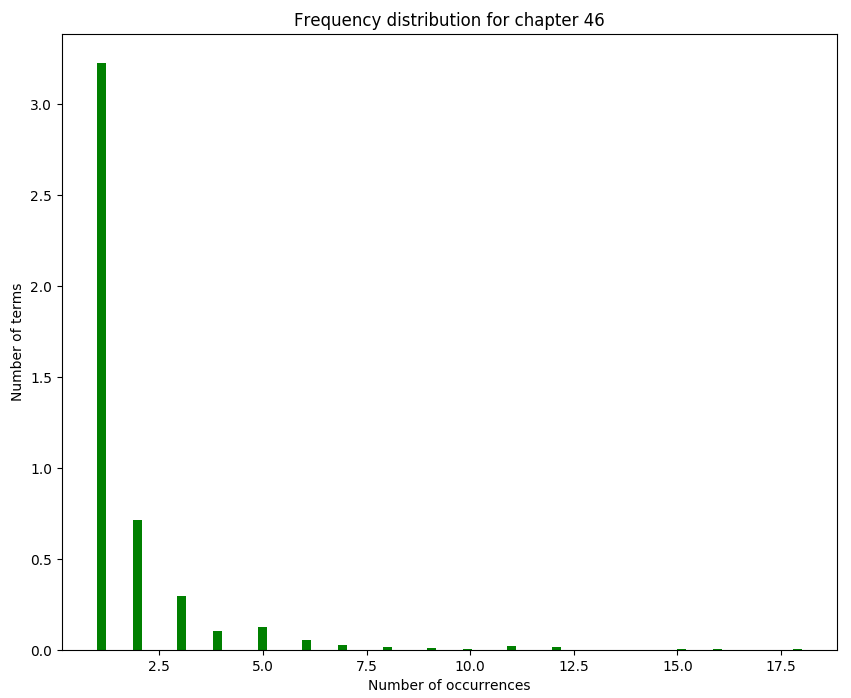
\includegraphics[width=0.75\textwidth]{./images/5-chapter_wise-frequency.png}
		\end{minipage}
		\hfill
		\begin{minipage}{0.45\linewidth}
			\centering
			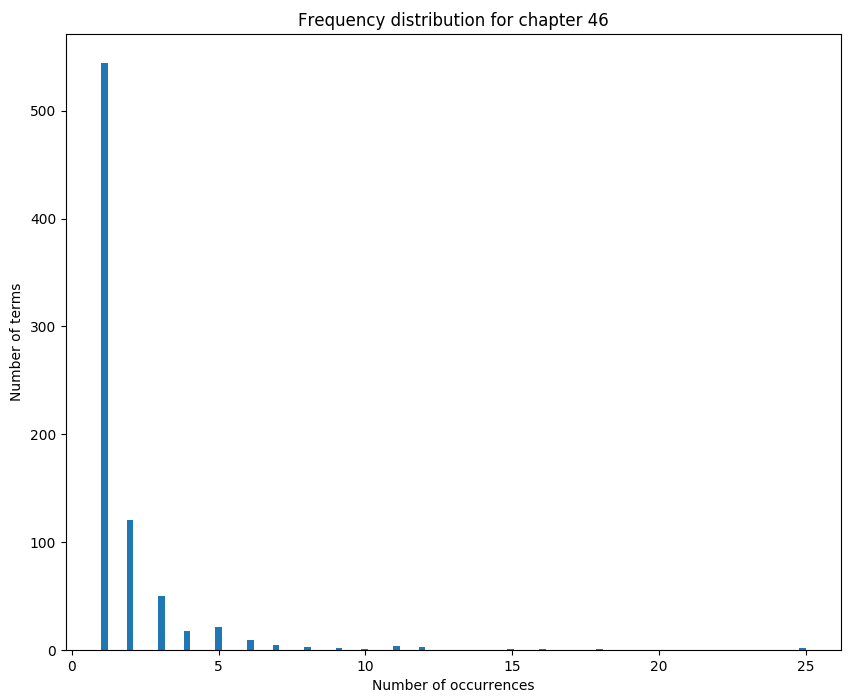
\includegraphics[width=0.75\textwidth]{./images/6-chapter_wise-frequency.png}
			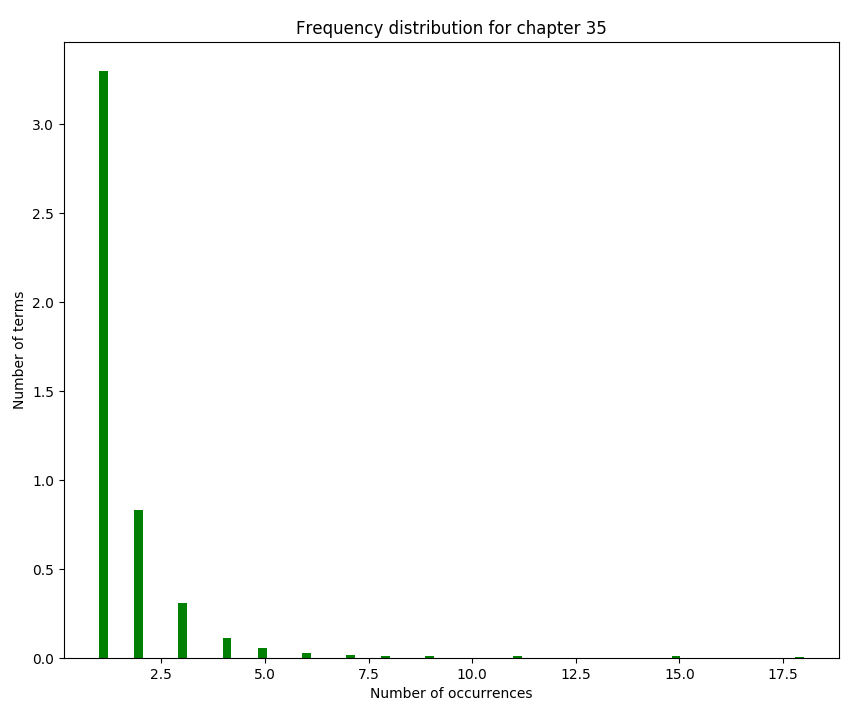
\includegraphics[width=0.75\textwidth]{./images/7-chapter_wise-frequency.png}
			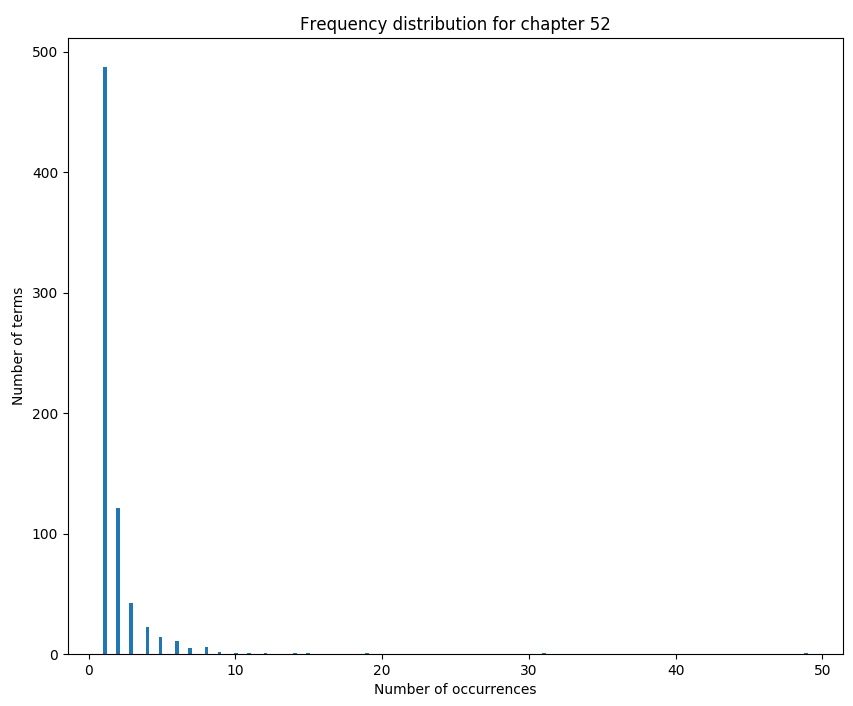
\includegraphics[width=0.75\textwidth]{./images/8-chapter_wise-frequency.png}
			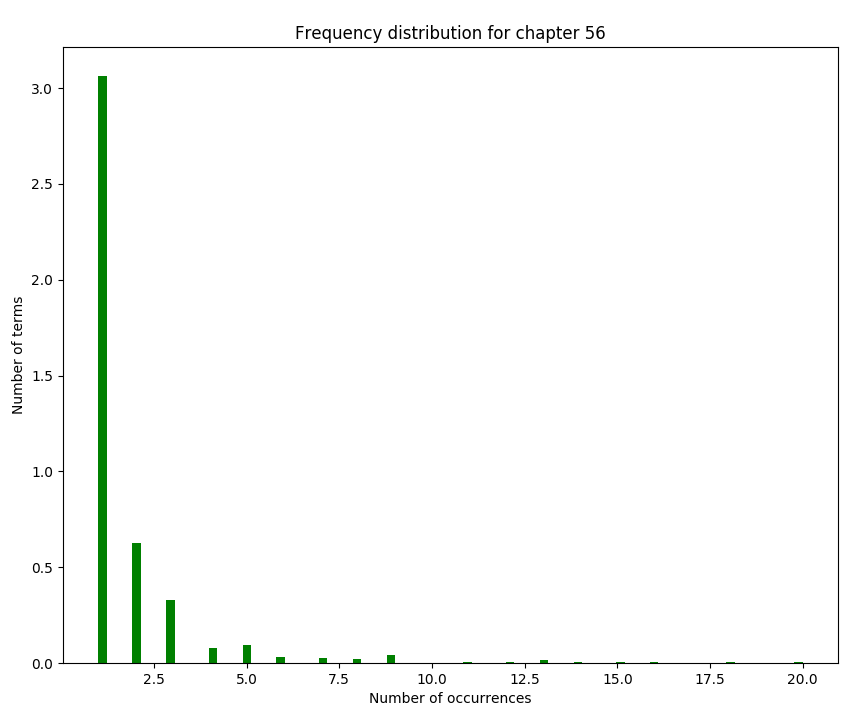
\includegraphics[width=0.75\textwidth]{./images/9-chapter_wise-frequency.png}
			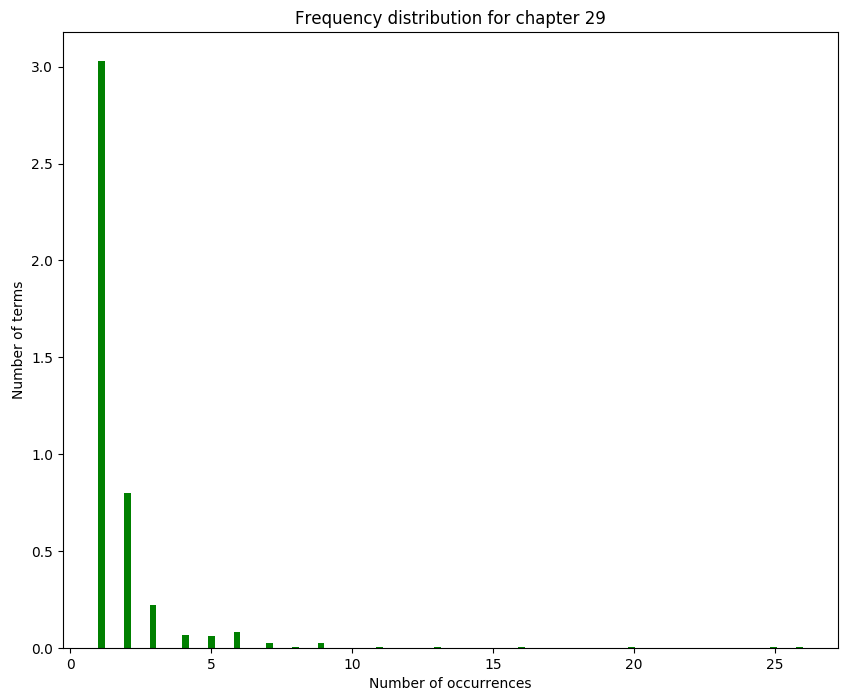
\includegraphics[width=0.75\textwidth]{./images/10-chapter_wise-frequency.png}
		\end{minipage}
		\caption{Each plot from top to bottom represents a different chapter.\newline{}These are (ordered from top to bottom): 62, 18, 43, 47, 16, 46, 53, 52, 35, 56}
	\end{figure}
\end{flushleft}

\subsection{Top 20 words}
\begin{flushleft}
	The top 20 words (based on frequency) obtained for 10 chapters are as follows:
	\begin{center}
		\begin{tabular}{|p{0.08\textwidth}|p{0.37\textwidth}||p{0.08\textwidth}|p{0.37\textwidth}|}
			\hline
			Chapter Number & Top 20 Words & Chapter Number & Top 20 Words \\
			\hline
			\hline
			62 & \lq\lq, \rq\rq, mr, elizabeth, could, would, said, darcy, bennet, much, must, sister, miss, one, lady, jane, bingley, know, though, never &
			18 & mr, \lq\lq, \rq\rq, darcy, elizabeth, could, said, bingley, though, wickham, sister, say, lady, much, must, may, would, time, collins, dance\\
			\hline
			43 & \lq\lq,\rq\rq, mr, elizabeth, could, gardiner, said, might, master, darcy, thought, much, every, know, room, aunt, time, little, seen, good & 
			47 &  \lq\lq, \rq\rq, could, know, elizabeth, lydia, well, mr, jane, give, think, must, u, would, might, wickham, hope, much, one, colonel  \\
			\hline
			16 & \lq\lq, \rq\rq, mr, darcy, elizabeth, wickham, could, said, lady, man, much, father, pride, manner, collins, phillips, nothing, know, believe, catherine &
			46 & \lq\lq, \rq\rq could, mr, lydia, elizabeth, must, would, letter, though, nothing, one, know, darcy, u, never, first, colonel, well, gardiner\\
			\hline
			53 & \lq\lq, \rq\rq, mr, said, know, could, elizabeth, bingley, bennet, sister, jane, come, see, without, one, soon, must, daughter, looked, never &
			52 & \lq\lq, \rq\rq, would, mr, wickham, could, must, uncle, time, darcy, lydia, sister, know, done, every, much, never, soon, u, though  \\
			\hline
			35 & mr, sister, could, \lq\lq, wickam, father, must, would, last, soon, letter, year, one, feeling, may, shall, every, though, two, friend   &
			56 & \lq\lq, \rq\rq, elizabeth, bennet, lady, miss, catherine, would, mr, ladyship, nephew, shall, must, know, said, say, make, well, mother, family \\
			\hline
		\end{tabular}
	\end{center}
\end{flushleft}
\newpage

\section{Plots, Top 20 words and Observations - Complete Book}
\subsection{Metric: Frequency}
\subsubsection{Distribution Plot}
\begin{flushleft}
	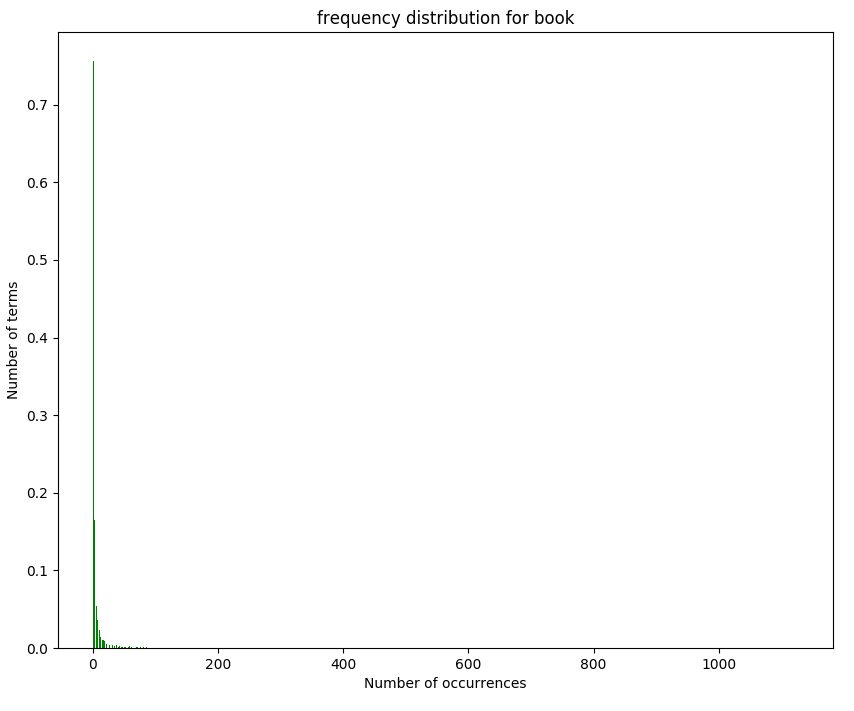
\includegraphics[width=0.75\textwidth]{./images/frequency-distribution-book.png}
\end{flushleft}
\subsubsection{Top 20 words}
\begin{flushleft}
	\lq\lq, \rq\rq, mr, elizabeth, could, would, said, darcy, bennet, much, must, sister, miss, one, lady, jane, bingley, know, though, time
\end{flushleft}
\subsubsection{Observations}
TODO

\newpage
\subsection{Metric: Entropy}
\subsubsection{Distribution Plot}
\begin{flushleft}
	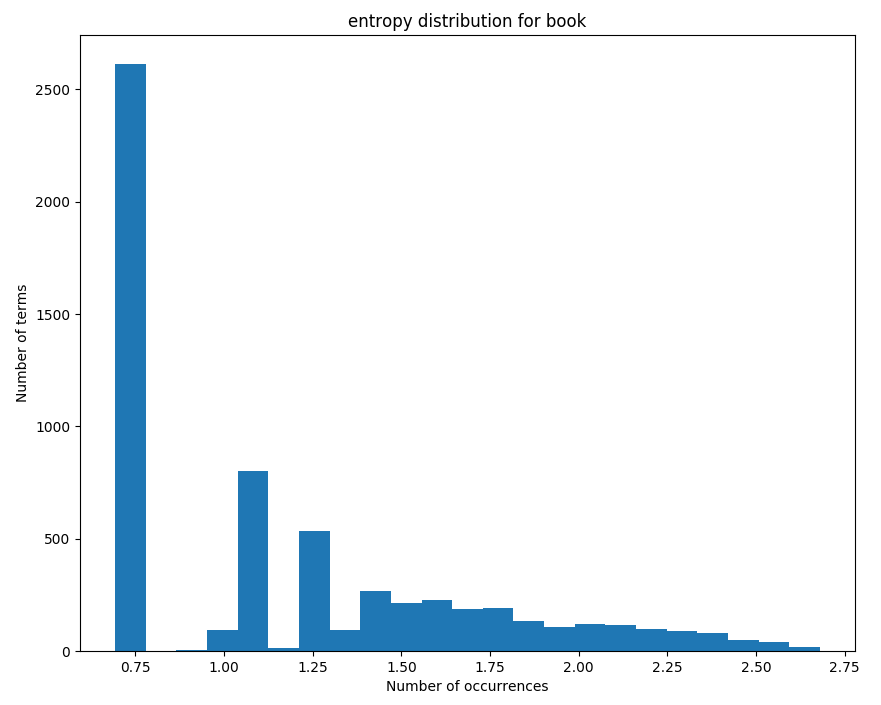
\includegraphics[width=0.75\textwidth]{./images/entropy-distribution-book.png}
\end{flushleft}
\subsubsection{Top 20 words}
\begin{flushleft}
    would, mr, much, could, elizabeth, little, one, without, great, \lq\lq, soon, day, \rq\rq, said, must, time, never, family, see, however \\
\end{flushleft}
\subsubsection{Scatter Plot}
\begin{flushleft}
	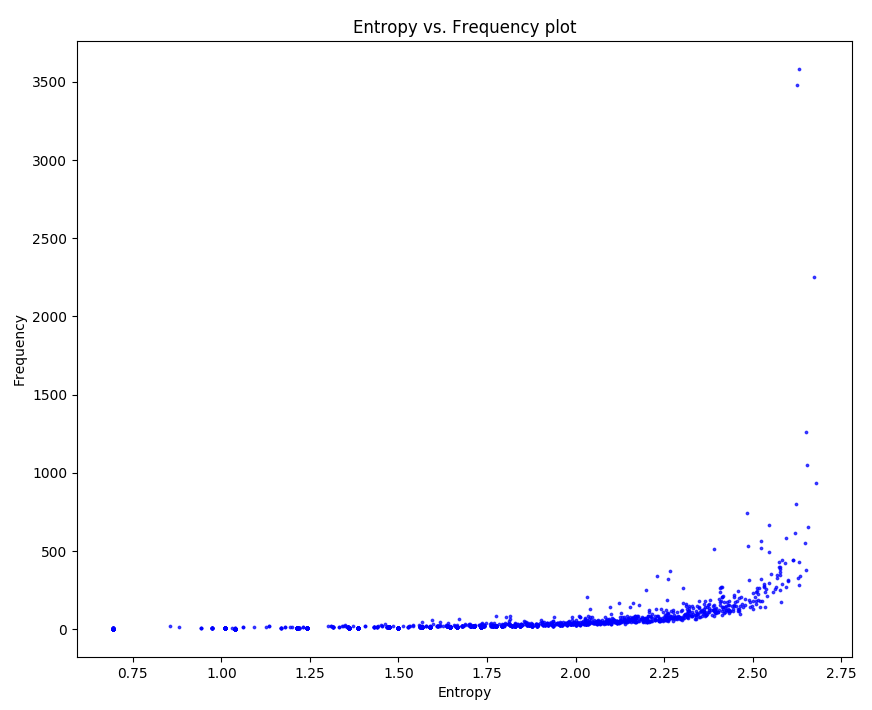
\includegraphics[width=0.75\textwidth]{./images/scatter-plot.png}
\end{flushleft}
\subsubsection{Observations}
TODO

\newpage
\subsection{Metric: THE VISHWAK :) }
\subsubsection{Explanation}
TODO
\subsubsection{Advantages/ Disadvantages}
TODO
\subsubsection{Top 20 words}
\begin{flushleft}
    mr, would, \lq\lq, much, elizabeth, \rq\rq, sister, said, miss, one, must, without, little, soon, every, though, however, could, know, time
\end{flushleft}
\subsubsection{Observations}
TODO

\end{document}